\documentclass[11pt,a4paper,oneside]{article}
\usepackage[utf8]{inputenc}
\usepackage{amsmath}
\usepackage{amsfonts}
\usepackage{amssymb}
\usepackage{graphicx}
\usepackage{color}
\usepackage {tikz}
\usetikzlibrary {er}
\usepackage[left=2.00cm, right=2.00cm, top=1.00cm]{geometry}
\graphicspath{{./}}

\begin{document}
	\title{DS 256 - Scalable Systems for Data Science \\ Assignment 1}
	\author{Shriram R. \\ M Tech (CDS) \\ 06-02-01-10-51-18-1-15763}
	\maketitle
	
	\section{Introduction}
	Distributed graph algorithms were implemented using Apache Spark RDD and Giraph vertex centric API. Strong and weak scaling experiments were performed using different public graph datasets to study the performance of these platforms in terms of different metrics. The following sections cover the experimental setup, plots and analysis in detail.  
	
	\section{Algorithms}
	The following four algorithms have been implemented for this assignment. Some brief notes on them is provided below,
	
	\subsection{Weakly Connected Components}
	This is an iterative algorithm which converges once all the vertices in each weakly connected component reach the same value. The graphs were processed as undirected for this algorithm. The no. of steps would be roughly the diameter of the undirected graph
	
	\subsection{Conductance}
	This is the only single pass algorithm out of all four. The graphs were processed as undirected. In each execution, approximately $\frac{1}{3}^{rd}$ of the vertices were marked as IN in random fashion and the remaining were marked as OUT. This is to avoid a input vertex list for the experiments.
	
	\subsection{PageRank}
	This algorithm is iterative and is made to run till convergence. The tolerance was set to $1\%$ and the weight was set to $0.85$ for all the experiments. The graphs were treated as directed graph. The no of iterations depend on the structure of the graph and it is guaranteed to converge. 
	
	\subsection{Spanning Tree}
	This algorithm is also iterative and runs till the spanning tree is formed. The graphs were processed as undirected and a source vertex (Vertex ID = 1) is given as input to start the spanning tree search. The no. of iterations should be close to that of weakly connected components.
	     
    \section{Experimental Setup}
    
    \subsection{Hardware}
    Experiments were performed on a commodity cluster having 24 compute nodes. Each node has a 8-core AMD Opteron 3380 processor clocked at 2.6Ghz along with 32GB RAM and 2TB HDD and runs Ubuntu 16.04 LTS (64 bit) with Linux 4.4.0-139-generic. The nodes are connected through a Gigabit Ethernet switch.
    
    \subsection{HDFS and Apache Spark}
    The cluster is provisioned with Apache Hadoop 3.1.1. HDFS environment has a capacity of 1.32TB with block size 128MB, replication factor of 2 and heartbeat delay of 3s. The global configuration of Spark for all experiments is 3 executor cores per executor (containers) having 8GB of memory. The Driver memory was set to 512MB. Apache YARN was used to coordinate the job execution and jobs were submitted through cluster mode. Experiment specific detail if any is provided below.
    
    \subsection{Apache Giraph}
    The cluster is provisioned with Apache Giraph version 1.3.0. Each worker runs with 8 concurrent execution threads. The graphs are partitioned using Giraph's native hash partitioning. Checkpointing of the execution state and out-of-core execution was turned off for all experiments. The log level was set to debug and the Giraph metrics system was enabled. Apache YARN was used as the resource manager. YARN heap size was set to 12000 MB. 
    
    \subsection{Dataset}
    Experiments were run on the following three datasets. More datasets were not explored due to logistic constraints. The following table provides a summary of the graph datasets used,
    \begin{center}
    \begin{tabular}{|c|c|c|c|c|}
    	\hline 
    	\textbf{Dataset} & \textbf{Vertices $|V|$}  & \textbf{Edges $|E|$} & \textbf{Size (MB)} & \textbf{Input Format}\\
    	\hline
    	CITP & 3,774,768 & 16,518,948 & 280 & Edge List (TSV) \\
    	\hline
    	LIVJ & 4,847,571 & 68,993,773 & 1080 & Edge List (TSV) \\
    	\hline
    	ORKUT & 3,072,441 & 117,185,083 & 1769 & Edge List (TSV)\\
    	\hline
    \end{tabular}
    \end{center}
    	
    \section{Results}
    
    \begin{center}
    	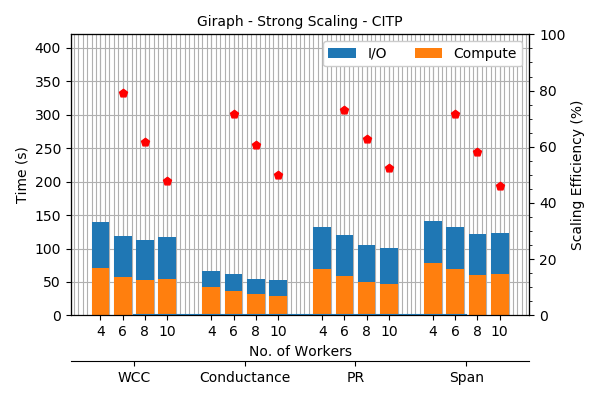
\includegraphics[scale=0.6]{1.png}		
    \end{center}

    \begin{center}
    	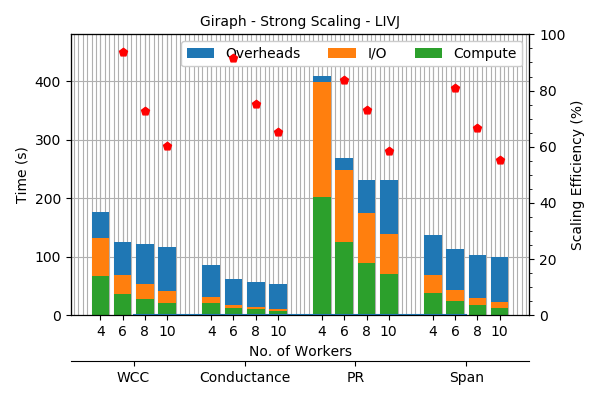
\includegraphics[scale=0.6]{2.png}		
    \end{center}

    \begin{center}
    	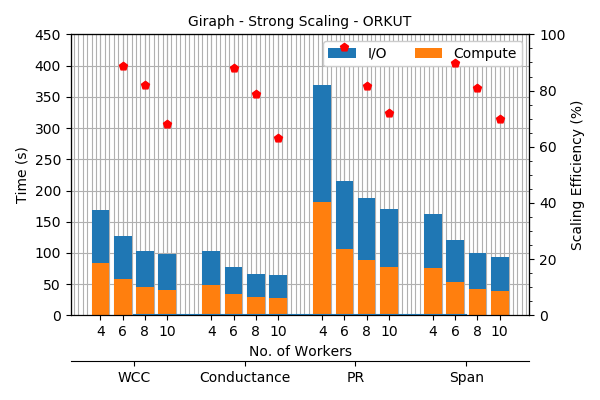
\includegraphics[scale=0.6]{3.png}		
    \end{center}

    \begin{center}
    	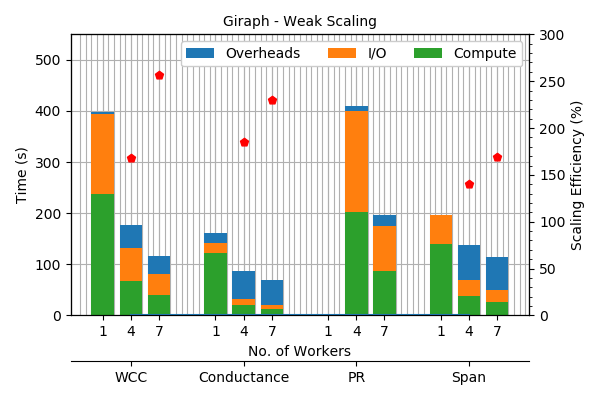
\includegraphics[scale=0.6]{4.png}		
    \end{center}
        
    \section{References}
    \begin{list}{}{}
    	\item
    	\item
    \end{list}  
    
\end{document}